\documentclass[table]{beamer}
\mode<presentation>
{
  \usetheme{Berkeley}
}

% 设定英文字体
\usepackage{fontspec}
\setmainfont{Arial}
%\setmainfont{Times New Roman}
\setsansfont{Arial}
\setmonofont{Courier New}

% 设定中文字体
\usepackage[BoldFont,SlantFont,CJKchecksingle,CJKnumber]{xeCJK}
\setCJKmainfont[BoldFont={Adobe Heiti Std},ItalicFont={Adobe Kaiti Std}]{Adobe Song Std}

\usepackage{setspace}
\usepackage{booktabs}
\usepackage{colortbl,xcolor}
\usepackage{hyperref}

% 插入图片
\usepackage{graphicx}
% 指定存储图片的路径(当前目录下的figures文件夹)
\graphicspath{{figures/}}

% 可能用到的包
\usepackage{amsmath,amssymb}
\usepackage{multimedia}
\usepackage{multicol}

% item逐步显示时,使已经出现的item、正在显示的item、将要出现的item呈现不同颜色
\def\hilite<#1>{
 \temporal<#1>{\color{gray}}{\color{blue}}
    {\color{blue!25}}
}

% 在表格、图片等得标题中显示编号
\setbeamertemplate{caption}[numbered]


\logo{
\includegraphics[height=0.12\textwidth]{bnu_tiny}}

\title[简要标题]{论文标题}
%\subtitle{Optional Subtitle}

\author[作者]{作者1\inst{1} \and 作者2\inst{2}}
\institute[北京师范大学]
{
    \inst{1}
    大数据与物联网实验室 \\
    信息科学与技术学院
    \and
    \inst{2}
    虚拟现实实验室 \\
    信息科学与技术学院
}
\date{2015年5月23日}
\subject{Theoretical Computer Science}

\AtBeginSubsection[]
{
  \begin{frame}<beamer>
	%\setcounter{tocdepth}{2}
    \tableofcontents[currentsection,currentsubsection]
  \end{frame}
}

\numberwithin{equation}{section}%使公式编号关联至章节
\setbeamertemplate{theorems}[numbered]%显示定理编号

\begin{document}

\begin{frame}
  \titlepage
\end{frame}

\begin{frame}{大纲}
  \tableofcontents
\end{frame}

%%%% 第一章
\section{第一章}
\subsection{1.1}
\frame{
    \frametitle{带编号的公式示例}
    \begin{equation}
    \begin{split}
	a_{i}^{T}X \leq b_{i},\ i=1,2,...,n\\
	0 \leq x_{i} \leq P_{i},\ i=1,2,..  .,N
    \end{split}
    \end{equation}
}

\subsection{1.2}
\frame{
    \frametitle{各条依次显示示例}
    \begin{itemize}
	\item <1-> 第一条\\
	\item <2-> 第二条\\
    ......
    \end{itemize}
}

\frame{
    \frametitle{带编号列表示例}
    \begin{enumerate}
    \item aaa
    \item bbb\\
    ...
    \end{enumerate}
}



%%%%%%%%%%%%%%%%%%%%%%%%%%%%%第二章%%%%%%%%%%%%%%%%%%%%%%%%%%%%%%%%% 
\section{第二章}
\subsection{2.1}
\begin{frame}{插图示例}
    \centering{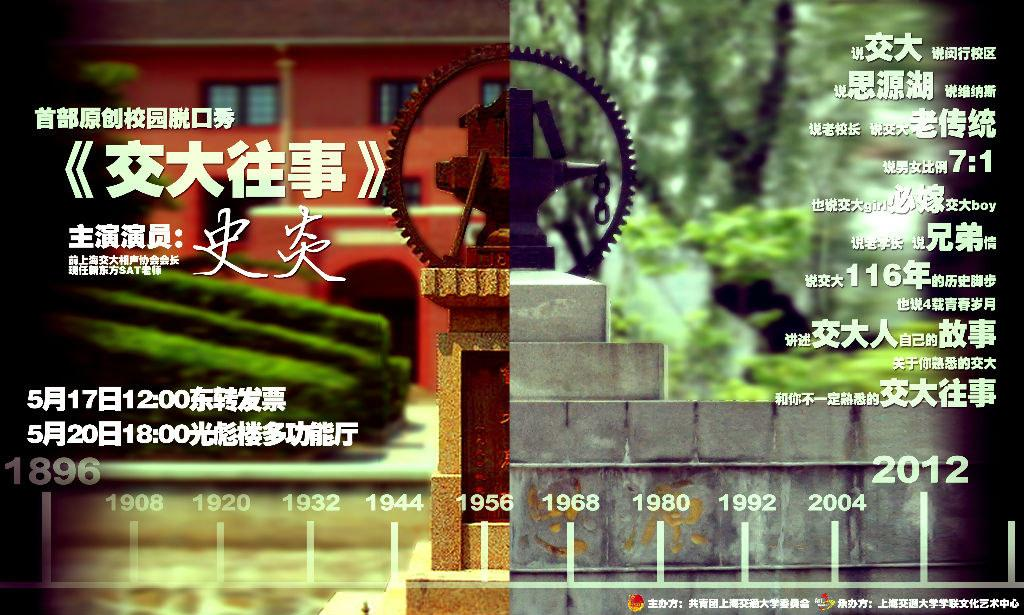
\includegraphics[width=10cm]{jdws.jpg}}%图片放于figures文件夹
\end{frame}

\subsection{2.2}
\frame{
    \frametitle{显示公式示例}
     \begin{theorem}[定理名称]\label{dl}%可以用\label{}和ref{}引用定理
    XXX定理
    \end{theorem}
}

\subsection{2.3}
\begin{frame}{表格示例}
% Table generated by Excel2LaTeX from sheet 'Sheet1' 推荐用excel2latex直接生成表格的tex代码
\begin{table}[htbp]
  \centering
  \caption{表格标题}
    \begin{tabular}{rrrrr}
    \addlinespace
    \toprule
          & c1    & c2    & c3    & c4 \\
    \midrule
    r1    & a     & e     & i     & m \\
    r2    & b     & f     & j     & n \\
    r3    & c     & g     & k     & o \\
    r4    & d     & h     & l     & p \\
    \bottomrule
    \end{tabular}%
  \label{tab:addlabel}%
\end{table}%
\end{frame}

\section{First Main Section}


\subsection{Second Subsection}

% You can reveal the parts of a slide one at a time
% with the \pause command:
\begin{frame}{Second Slide Title}
  \begin{itemize}
  \item {
    First item.
    \pause % The slide will pause after showing the first item
  }
  \item {   
    Second item.
  }
  % You can also specify when the content should appear
  % by using <n->:
  \item<3-> {
    Third item.
  }
  \item<4-> {
    Fourth item.
  }
  % or you can use the \uncover command to reveal general
  % content (not just \items):
  \item<5-> {
    Fifth item. \uncover<6->{Extra text in the fifth item.}
  }
  \end{itemize}
\end{frame}

\section{Second Main Section}

\subsection{Another Subsection}

\begin{frame}{Blocks}
\begin{block}{Block Title}
You can also highlight sections of your presentation in a block, with it's own title
\end{block}
\begin{theorem}
There are separate environments for theorems, examples, definitions and proofs.
\end{theorem}
\begin{example}
Here is an example of an example block.
\end{example}
\end{frame}

% Placing a * after \section means it will not show in the
% outline or table of contents.
\section*{Summary}

\begin{frame}{Summary}
  \begin{itemize}
  \item
    The \alert{first main message} of your talk in one or two lines.
  \item
    The \alert{second main message} of your talk in one or two lines.
  \item
    Perhaps a \alert{third message}, but not more than that.
  \end{itemize}
  
  \begin{itemize}
  \item
    Outlook
    \begin{itemize}
    \item
      Something you haven't solved.
    \item
      Something else you haven't solved.
    \end{itemize}
  \end{itemize}
\end{frame}



% All of the following is optional and typically not needed. 
\appendix
\section<presentation>*{\appendixname}
\subsection<presentation>*{For Further Reading}

\begin{frame}[allowframebreaks]
  \frametitle<presentation>{For Further Reading}
    
  \begin{thebibliography}{10}
    
  \beamertemplatebookbibitems
  % Start with overview books.

  \bibitem{Author1990}
    A.~Author.
    \newblock {\em Handbook of Everything}.
    \newblock Some Press, 1990.
 
    
  \beamertemplatearticlebibitems
  % Followed by interesting articles. Keep the list short. 

  \bibitem{Someone2000}
    S.~Someone.
    \newblock On this and that.
    \newblock {\em Journal of This and That}, 2(1):50--100,
    2000.
  \end{thebibliography}
\end{frame}

\end{document}
